\documentclass[../admech.tex]{subfiles}
\begin{document}
\section{Disintegration of Particles}
The most simple case of collision that we might begin to investigate, is the decay of a particle with mass $M$ into two particles with masses $m_1,m_2$. Firstly considering the center of mass system (that we will call the \emph{cm} system), we immediately apply the conservation of energy and momentum to such case, and writing $p_0=\norm{p_1^\mu}_\mu=\norm{p_2^\mu}_\mu$, we must have
\begin{equation}
	E_{int}=E_{1,int}+E_{2,int}+\frac{p_0^2}{2m_1}+\frac{p_0^2}{2m_2}
	\label{eq:disencons}
\end{equation}
Where $p_0^2/2m_i$ is the kinetic energy of the $i$-th particle, and $E_{int}$ is the ``internal'' energy of the particles.\\
This process is possible only if the internal energy of the first particle is greater than the sum of the internal energies of the two particles, we call this the \emph{disintegration energy} $\epsilon$, and we must have
\begin{equation}
	\epsilon=E_{int}-E_{1,int}-E_{2,int}>0
	\label{eq:disen}
\end{equation}
Subsituting into \eqref{eq:disencons} we have a different definition for this energy
\begin{equation}
	\epsilon=\frac{p_0^2}{2}\left( \frac{1}{m_1}+\frac{1}{m_2} \right)=\frac{p_0^2}{2\mu}
	\label{eq:disenrmass}
\end{equation}
Where the reduced mass $\mu$ pops directly from the definition, where $\mu^{-1}=m_1^{-1}+m_2^{-1}$. The velocities of the particles in the cm system are really easy to find, and since $m_iv_i=p_0$ we have
\begin{equation}
	\left\{ \begin{aligned}
			v_1&=\frac{p_0}{m_1}\\
			v_2&=\frac{p_0}{m_2}
	\end{aligned}\right.
	\label{eq:velcmsysdecay}
\end{equation}
Obviously they'll be directed in opposite directions.\\
We now change to a new reference system where our main particle with mass $M$ moves with some velocity $V$, we will call this the \emph{laboratory} system (indicated as \emph{l}).\\
Considering only the first of the two resulting particles we have that in this transformation, if $v_0^\mu$ is the velocity in the cm system
\begin{equation}
	v^\mu=V^\mu+v_0^\mu\implies v^2_0=v^2+V^2+2vV\cos\theta
	\label{eq:decayspeedV}
\end{equation}
Where the $\cos\theta$ pops out from a scalar product, and indicates the angle between the direction of the velocity of the main particle and the decayed particle.\\
An easy and intriguing way that can be used to solve this kind of collision was given by L. D. Landau and E. M. Lifshits in the book \cite{landau1}, where we use geometry to get everything about the system.\\
\begin{enumerate}
	\item Begin by drawing a circle with radius $v_0$, draw a vector from the origin till the circle at an angle $\theta_0$, this will represent the vector $v_0$ and the angle in the cm system. The point where $v_0$ will touch the circumference will be the point $C$
	\item Draw a line of length $V$ from the origin and call the arrival point $A$, make this a vector by adding the verse, strictly from $A$ to the origin
	\item Draw a vector from $A$ to the point $C$, this will represent the vector $v$ in the l system. The angle between $v$ and $V$ is the angle $\theta$
\end{enumerate}
This gives immediately two cases. If $V<v_0$ the vector $V$ will be completely contained in the circle and the point $C$ can lay in every point of the circumference, i.e. $\theta,\theta_0\in[0,2\pi]$, instead if $V>v_0$ this is not true anymore, and there will be some $\theta_{max}$ that can be reached.\\
\begin{minipage}[c]{0.5\textwidth}
	\begin{figure}[H]
		\centering
		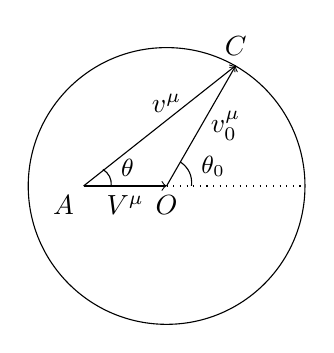
\begin{tikzpicture}
			\draw (0,0) circle (50pt);
			\draw[->] (0,0) -- (25pt,43.5pt) node[above] {$C$};
			\draw[->] (-30pt,0) -- (0,0);
			\draw[dotted] (0,0) -- (50pt,0);
			\node[below] at (-15pt,0) {$V^\mu$};
			\node[right] at (12.5pt,21.75pt) {$v_0^\mu$};
			\draw[->] (-30pt,0) -- (25pt,43.5pt);
			\node at (0,30pt) {$v^\mu$};
			\node[below left] at (-30pt,0) {$A$};
			\node[below] at (0,0) {$O$};
			\draw (5pt,8.66pt) to [bend left=30] (9pt,0);
			\node[above right] at (9pt,0) {\small$\theta_0$};
			\draw (-23pt,6pt) to [bend left=30] (-20pt,0);
			\node[above right] at (-20pt,0) {\small$\theta$};
		\end{tikzpicture}
		\caption{Collision circle for the case $V<v_0$}
		\label{fig:discirc1}
	\end{figure}
\end{minipage}
\begin{minipage}[c]{0.5\textwidth}
	\begin{figure}[H]
		\centering
		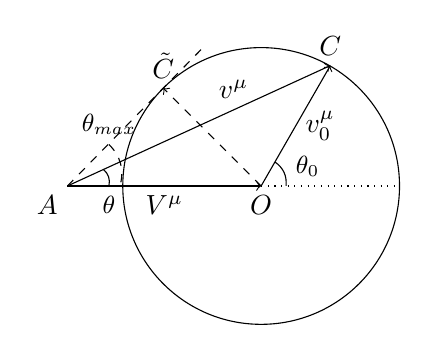
\begin{tikzpicture}
			\draw (0,0) circle (50pt);
			\draw[->] (0,0) -- (25pt,43.5pt) node[above] {$C$};
			\draw[->] (-70pt,0) -- (0,0);
			\draw[dotted] (0,0) -- (50pt,0);
			\node[below] at (-35pt,0) {$V^\mu$};
			\node[right] at (12.5pt,21.75pt) {$v_0^\mu$};
			\draw[->] (-70pt,0) -- (25pt,43.5pt);
			\node at (-10pt,35pt) {$v^\mu$};
			\node[below left] at (-70pt,0) {$A$};
			\node[below] at (0,0) {$O$};
			\draw (5pt,8.66pt) to [bend left=30] (9pt,0);
			\node[above right] at (9pt,0) {\small$\theta_0$};
			\draw[dashed] (-70pt,0) -- (-21pt,50pt);
			\draw (-57pt,6pt) to [bend left=30] (-55pt,0);
			\node[below] at (-55pt,0) {\small$\theta$};
			\draw[dashed] (-55pt,15pt) to [bend left=30] (-51pt,0);
			\node[above] at (-55pt,15pt) {\small$\theta_{max}$};
			\draw[dashed, ->] (0,0) -- (-35.36pt,35.36pt);
			\node[above] at (-35.36pt,35.36pt) {$\tilde{C}$};
		\end{tikzpicture}
		\caption{Collision circle for the case $V>v_0$. Note the presence of a maximum possible angle.}
		\label{fig:discirc2}
	\end{figure}
\end{minipage}\\
The maximum angle possible for the second case, where $V>v_0$ is calculated easily through trigonometry. We have
\begin{equation}
	V\sin(\theta_{max})=v_0\implies\sin(\theta_{max})=\frac{v_0}{V}
	\label{eq:maxangledis2p}
\end{equation}
Using the same circle it's possible to find the relations between the flight angles $\theta,\theta_0$ between the l system and the cm system. We have
\begin{equation}
	\left\{ \begin{aligned}
		v\sin\theta&=v_0\sin\theta_0\\
		v\cos\theta&=v_0\cos\theta_0+V
	\end{aligned}\right.
	\label{eq:falcmdiscoord}
\end{equation}
Thus giving us the following relation
\begin{equation}
	\tan\theta=\frac{v_0\sin\theta_0}{v_0\cos\theta_0+V}
	\label{eq:flightangldislcm}
\end{equation}
\subsection{Disintegration Into Multiple Particles}
In physics, while studying particle decays and disintegrations, it's common to actually have the disintegration of one particle into many particles. This problem in the cm system is obvious since resulting particles of the same kind have the same energy and their flight angle distribution is therefore isotropic in space.\\
This implies that the number of particles passing through some solid angle $\dd\Omega_0$ is proportional to the linear dimension of this element, $\dd\Omega_0/4\pi$. We therefore can write
\begin{equation}
	4\pi\dd{N_p}=2\pi\sin\theta_0\dd\theta_0=\dd\Omega_0\implies\dd{N_p}=\frac{1}{2}\sin\theta_0\dd\theta_0
	\label{eq:Ndisnumb0}
\end{equation}
Applying the transformation $v^\mu=v_0^\mu+V^\mu$ we move into the l system, and using equation \eqref{eq:decayspeedV}, we get
\begin{equation}
	\dd(\cos\theta_0)=\sin\theta_0\dd\theta_0=\frac{\dd(v^2)}{2v_0V}
	\label{eq:Ndiscml}
\end{equation}
Introducing the kinetic energy $T$ we can rewrite the previous equation as follows
\begin{equation}
	\sin\theta_0\dd\theta_0=\frac{\dd{T}}{2mv_0V}
	\label{eq:NdiscmlT}
\end{equation}
This gives us a constraint on the possible magnitude of the kinetic energy, which must be contained between these two values
\begin{equation}
	\left\{ \begin{aligned}
			T_{min}&=\frac{1}{2}m\left( v_0-V \right)^2\\
			T_{max}&=\frac{1}{2}m\left( v_0+V \right)^2
	\end{aligned}\right.
	\label{eq:NdisTminmax}
\end{equation}
Note that this gives us only an interval of possible energies in the l system, whereas in the cm system we end up having complete arbitrary values for $T$.\\
Consider now all resulting particles, minus one with mass $m_1$, as a whole system with mass $m_2$. Using the conservation of momentum we can say that the energy of particle $1$ must be
\begin{equation}
	T_{10}=\frac{p_0^2}{2m_1}
	\label{eq:part1T}
\end{equation}
Using the definition of $\epsilon$, \eqref{eq:disenrmass}, we can write this quantity differently
\begin{equation}
	T_{10}=\frac{M-m_1}{M}\left( \frac{1}{M+m_1}+\frac{1}{m_1} \right)\frac{p_0^2}{2}=\frac{M-m_1}{M}\left( E_{int}-E_{1int}-E_{2int} \right)=\frac{M-m_1}{M}\epsilon
	\label{eq:disenNpartT}
\end{equation}
Where $E_{int},M$ are respectively the internal energy and mass of the main particle \emph{before} the decay.
\section{Elastic Collisions}
A collision between two particles is called elastic if there are no changes in their states after the collision. The internal energy of the particles can be ignored thanks to the conservation of energy.\\
Indicating with the symbol $\square_0$ the quantities in the cm system, thanks to the conservation of momentum the particles will move with the following velocities in the cm system
\begin{equation}
	\left\{ \begin{aligned}
			v_{10}^\mu&=\frac{m_2}{m_1+m_2}v^\mu\\
			v_{20}^\mu&=-\frac{m_1}{m_1+m_2}v^\mu
	\end{aligned}\right.
	\label{eq:ecolv}
\end{equation}
Where $v^\mu=v_1^\mu-v_2^\mu=v\hat{n}_0^\mu$ is directed as the first particle's velocity.\\
Switching to the l system and accounting for the added velocity $V^\mu$ of the system we get, considering directly the new momentum of the two particles
\begin{equation}
	\left\{\begin{aligned}
			\tilde{p}_1^\mu&=\mu v\hat{n}_0^\mu+\frac{m_1}{m_1+m_2}(p_1^\mu+p_2^\mu)\\
			\tilde{p}_2^\mu&=-\mu v\hat{n}_0^\mu+\frac{m_2}{m_1+m_2}(p_1^\mu+p_2^\mu)
	\end{aligned}\right.
	\label{eq:ecolpl}
\end{equation}
Where the unsigned momentum is the momentum of the particle before the collision, and $\mu$ is the reduced mass\\
As for the disintegration of particles, we can represent an elastic collision in a collision circle as the following\\
\begin{minipage}[c]{0.5\textwidth}
	\begin{figure}[H]
		\centering
		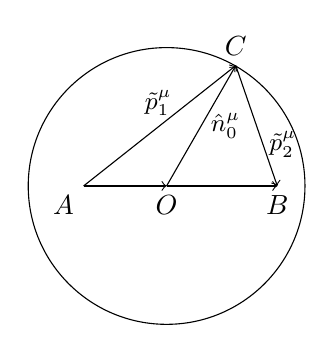
\begin{tikzpicture}
			\draw (0,0) circle (50pt);
			\draw[->] (0,0) -- (25pt,43.5pt) node[above] {$C$};
			\draw[->] (-30pt,0) -- (0,0);
			\draw[->] (0,0) -- (40pt,0) node[below] {$B$};
			\draw[->] (25pt,43.5pt) -- (40pt,0) ;
%			\node[below] at (-15pt,0) {$V^\mu$};
			\node[right] at (12.5pt,21.75pt) {\small$\hat{n}_0^\mu$};
			\draw[->] (-30pt,0) -- (25pt,43.5pt);
			\node at (-3pt,30pt) {\small$\tilde{p}_1^\mu$};
			\node at (42pt,15pt) {\small$\tilde{p}_2^\mu$};
			\node[below left] at (-30pt,0) {$A$};
			\node[below] at (0,0) {$O$};
%			\draw (5pt,8.66pt) to [bend left=30] (9pt,0);
%			\node[above right] at (9pt,0) {\small$\theta_0$};
%			\draw (-23pt,6pt) to [bend left=30] (-20pt,0);
%			\node[above right] at (-20pt,0) {\small$\theta$};
		\end{tikzpicture}
		\caption{Example of a collision circle for an elastic collision}
		\label{fig:exeecolcirc}
	\end{figure}
\end{minipage}
\begin{minipage}[c]{0.5\textwidth}
\begin{equation}
	\left[ \begin{aligned}
			\overline{OC}&=\mu v^\mu\\
			\overline{AO}&=\frac{m_1}{m_1+m_2}(p_1^\mu+p_2^\mu)\\
			\overline{OB}&=\frac{m_2}{m_1+m_2}\\
			\overline{AB}&=p_1^\mu\\
			\overline{AC}&=\tilde{p}_1^\mu\\
			\overline{CB}&=\tilde{p}_2^\mu\\
			\frac{\norm{\overline{AO}}}{\norm{\overline{OB}}}&=\frac{m_1}{m_2}
	\end{aligned}\right.
\end{equation}
\end{minipage}\\
As in the figure the vector $\hat{n}_0^\mu$ lays on the direction of the segment $OC$. The vectors going from the points $A$ to the point $C$ and from $C$ to $B$ represent respectively the impulses of the two particles after the collision. If both are fixed, so must be the radius of the circumference and both points $A,B$, while the point $C$ can instead lay wherever on the circumference\\
\begin{minipage}[c]{0.5\textwidth}
	\begin{figure}[H]
		\centering
		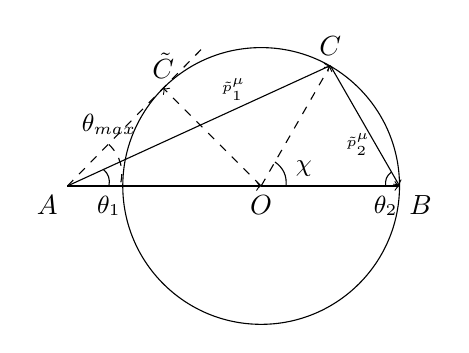
\begin{tikzpicture}
			\draw (0,0) circle (50pt);
			\draw[dashed,->] (0,0) -- (25pt,43.5pt) node[above] {$C$};
			\draw[->] (-70pt,0) -- (0,0);
			\draw[->] (0,0) -- (50pt,0) node[below right] {$B$};
			\draw[->] (25pt,43.5pt) -- (50pt,0);
%			\node[below] at (-35pt,0) {$V^\mu$};
%			\node[right] at (12.5pt,21.75pt) {\tiny$\hat{n}_0^\mu$};
			\draw[->] (-70pt,0) -- (25pt,43.5pt);
			\node at (-10pt,35pt) {\tiny$\tilde{p}_1^\mu$};
			\node at (35pt,15pt) {\tiny$\tilde{p}_2^\mu$};
			\node[below left] at (-70pt,0) {$A$};
			\node[below] at (0,0) {$O$};
			\draw (5pt,8.66pt) to [bend left=30] (9pt,0);
			\node[above right] at (9pt,0) {\small$\chi$};
			\draw[dashed] (-70pt,0) -- (-21pt,50pt);
			\draw (-57pt,6pt) to [bend left=30] (-55pt,0);
			\node[below] at (-55pt,0) {\small$\theta_1$};
			\draw[dashed] (-55pt,15pt) to [bend left=30] (-51pt,0);
			\node[above] at (-55pt,15pt) {\small$\theta_{max}$};
			\draw[dashed, ->] (0,0) -- (-35.36pt,35.36pt);
			\node[above] at (-35.36pt,35.36pt) {$\tilde{C}$};
			\draw (45pt,0) to [bend left=30] (47pt,5pt);
			\node[below] at (45pt,0) {\small$\theta_2$};
		\end{tikzpicture}
		\caption{Collision circle for an elastic collision between a moving particle and a particle at rest $m_1>m_2$.}
		\label{fig:ecolcirc1}
	\end{figure}
\end{minipage}
\begin{minipage}[c]{0.5\textwidth}
	A second case is if one of the two particles is at rest before the collision. Supposing that $m_2$ is at rest, we have that the point $B$ must lay on the circumference, since the segment $AB$ must coincide with the impulse $p_1^\mu$.
\end{minipage}\\
\begin{minipage}[c]{0.5\textwidth}
	There can be two main cases here, one where $m_1<m_2$ as in fig. \eqref{fig:ecolcirc1} and therefore the point $A$ lays on the inside of the circle and $C$ is free, and a second where $m_1>m_2$ as in fig. \eqref{fig:ecolcirc2} and $A$ is outside the circumference
\end{minipage}
\begin{minipage}[c]{0.5\textwidth}
	\begin{figure}[H]
		\centering
		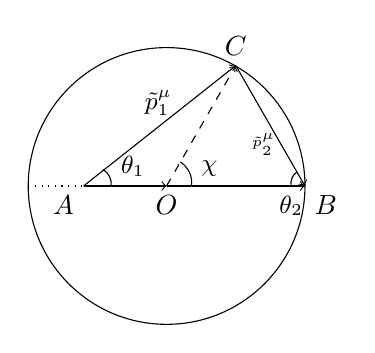
\begin{tikzpicture}
			\draw (0,0) circle (50pt);
			\draw[dashed,->] (0,0) -- (25pt,43.5pt) node[above] {$C$};
			\draw[->] (-30pt,0) -- (0,0);
			\draw[->] (0,0) -- (50pt,0) node[below right] {$B$};
			\draw[->] (25pt,43.5pt) -- (50pt,0);
%			\draw[dotted] (35pt,0) -- (50pt,0);
%			\node[below] at (-15pt,0) {$V^\mu$};
%			\node[right] at (12.5pt,21.75pt) {\small$\hat{n}_0^\mu$};
			\draw[->] (-30pt,0) -- (25pt,43.5pt);
			\node at (-3pt,30pt) {\small$\tilde{p}_1^\mu$};
			\node at (35pt,15pt) {\tiny$\tilde{p}_2^\mu$};
			\node[below left] at (-30pt,0) {$A$};
			\draw[dotted] (-50pt,0) -- (-30pt,0);
			\node[below] at (0,0) {$O$};
			\draw (5pt,8.66pt) to [bend left=30] (9pt,0);
			\node[above right] at (9pt,0) {\small$\chi$};
			\draw (-23pt,6pt) to [bend left=30] (-20pt,0);
			\node[above right] at (-20pt,0) {\small$\theta_1$};
			\draw (45pt,0) to [bend left=30] (47pt,5pt);
			\node[below] at (45pt,0) {\small$\theta_2$};
		\end{tikzpicture}
		\caption{Collision circle for the same collision where $m_1<m_2$}
		\label{fig:ecolcirc2}
	\end{figure}
\end{minipage}\\
The angles $\theta_1,\theta_2$ depicted in both figures represent the deflection of both particles from the initial direction of the incoming particle. The angle $\chi$, analogously to the angle $\theta_0$ represents the deflection of the incoming particle in the system cm. Both angles $\theta_1,\theta_2$ can be expressed in terms of $\chi$ using trigonometry, yielding
\begin{equation}
	\tan\theta_1=\frac{m_2\sin\chi}{m_1+m_2\cos\chi}\qquad\theta_2=\frac{\pi-\chi}{2}
	\label{eq:ecol12chi}
\end{equation}
The magnitudes of both velocities can also be expressed using the angle $\chi$, as
\begin{equation}
	\tilde{v}_1=\frac{1}{m_1+m_2}\sqrt{m_1^2+m_2^2+2m_1m_2\cos\chi}\qquad\tilde{v}_2=\frac{2m_1v}{m_1+m_2}\sin\left( \frac{\chi}{2} \right)
	\label{eq:ecolv12chi}
\end{equation}
From these two diagrams we can also extrapolate another constraint to the angle $\theta=\theta_1+\theta_2$, we must have therefore
\begin{equation}
	\begin{dcases}
		\theta>\frac{\pi}{2}&m_1<m_2\\
		\theta<\frac{\pi}{2}&m_1>m_2\\
	\end{dcases}
	\label{eq:thetaecol}
\end{equation}
Another case possible is that the particles collide head on, where $\chi=\pi$, forcing the new momenta of each particle to be equal and opposite or either in the same direction between points $A$ and $O$. Looking back at the dependence between the velocities and $\chi$, this is the maximum value possible for $\tilde{v}_2$. The maximum possible energy of such collision is therefore
\begin{equation}
	\tilde{E}_{2,max}=\frac{m_2\tilde{v}_{2,max}^2}{2}=\frac{4\mu}{m_1+m_2}E_1
	\label{eq:ecolE2max}
\end{equation}
Where we used the law of conservation of energy in order to tie this with the energy of the incoming projectile $E_1$.\\
The maximum angle possible $\theta_{max}$ shown in the diagram for the collision with a projectile with mass $m_1>m_2$ is calculated directly with trigonometry as follows
\begin{equation}
	\sin\theta_{max}=\frac{OC}{OA}=\frac{m_1}{m_2}
	\label{eq:thetamaxecol}
\end{equation}\\
The final and most simple case of elastic collision is the one between the projectile and target of both equal mass. Both points $A,B$ lay on the circumference and the angles $\theta_1,\theta_2$ are mutually orthogonal
\begin{minipage}[c]{0.5\textwidth}
	\begin{figure}[H]
		\centering
		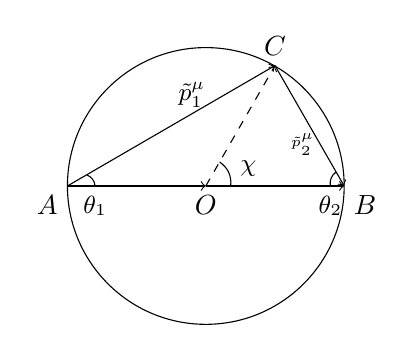
\begin{tikzpicture}
			\draw (0,0) circle (50pt);
			\draw[dashed,->] (0,0) -- (25pt,43.5pt) node[above] {$C$};
			\draw[->] (-50pt,0) -- (0,0);
			\draw[->] (0,0) -- (50pt,0) node[below right] {$B$};
			\draw[->] (25pt,43.5pt) -- (50pt,0);
			\draw[->] (-50pt,0) -- (25pt,43.5pt);
			\node at (-5pt,33pt) {\small$\tilde{p}_1^\mu$};
			\node at (35pt,15pt) {\tiny$\tilde{p}_2^\mu$};
			\node[below left] at (-50pt,0) {$A$};
			\node[below] at (0,0) {$O$};
			\draw (5pt,8.66pt) to [bend left=30] (9pt,0);
			\node[above right] at (9pt,0) {\small$\chi$};
			\draw (-43pt,4pt) to [bend left=30] (-40pt,0);
			\node[below] at (-40pt,0) {\small$\theta_1$};
			\draw (45pt,0) to [bend left=30] (47pt,5pt);
			\node[below] at (45pt,0) {\small$\theta_2$};
		\end{tikzpicture}
		\caption{Collision circle for an elastic collision where $m_1=m_2$}
		\label{fig:ecolcirceq}
	\end{figure}
\end{minipage}
\begin{minipage}[c]{0.5\textwidth}
	\begin{equation*}
		\left[ \begin{aligned}
				\theta_1&=\frac{\chi}{2}\\
				\tilde{v}_1&=v\cos\left( \frac{\chi}{2} \right)\\
				\theta_2&=\frac{\pi-\chi}{2}\\
				\tilde{v}_2&=v\sin\left( \frac{\chi}{2} \right)
			\end{aligned}\right.
	\end{equation*}
\end{minipage}
\section{Particle Scattering}
As seen in the previous section, for getting the angle $\chi$ and therefore a complete definition of the problem it's necessary to solve the equations of motion with some interaction law between the particles.\\
It's possible to consider an equivalent, and general, case where a particle of mass $m$ gets deflected from a central force field $\pot(r)$ (as if it was centered in the center of mass of the 2 colliding particles).\\
As already known, the trajectory of the particles in a central field are symmetric to a line from the center to the closest point of the particle, and the asymptotes of the orbit intersecate this line at the same angles $\varphi_0$. The angle of scattering $\chi$ will therefore be
\begin{equation}
	\chi=\abs{\pi-2\varphi_0}
	\label{eq:scattang0}
\end{equation}
The angle $\varphi_0$ is determined by the integral
\begin{equation}
	\varphi_0=\int_{r_{min}}^{\infty}\frac{1}{r^2\sqrt{2m(E-\pot(r))-\frac{L^2}{r^2}}}\dd{r}
	\label{eq:phi0scattang}
\end{equation}
Where $r_{min}$ is the closest distance from the center, found as
\begin{equation}
	\sqrt{2m(E-\pot(r_{min})-\frac{L^2}{r_{min}^2}}=0
	\label{eq:mindistscattang}
\end{equation}
For an infinite motion, it's useful to consider directly the speed at $\infty$, $v_\infty$ and a \emph{collision parameter} $\rho$, where
\begin{equation}
	\left\{ \begin{aligned}
			v_\infty&=\sqrt{\frac{2E}{m}}\\
			\rho&=\frac{L}{mv_\infty}
	\end{aligned}\right.
	\label{eq:vinfrhoscatt}
\end{equation}
Therefore, rewriting the integral \eqref{eq:phi0scattang}
\begin{equation}
	\varphi_0(\rho,v_\infty)=\int_{r_{min}}^{\infty}\frac{\rho}{r^2\sqrt{1-\frac{\rho^2}{r^2}-\frac{2\pot(r)}{mv_\infty^2}}}\dd{r}
	\label{eq:phi0new}
\end{equation}
Which gives us the dependence of $\chi$ to those two parameters.\\
In the case that there is actually a beam of particles getting scattered, this gets a bit more difficult since each particle of the beam has its own $\rho_i$.\\
Call $\dd N$ the density of particles getting scattered with some angle in $[\chi,\chi+\dd\chi]$. We define the \emph{scattering cross-section} $\dd\sigma$ as
\begin{equation}
	\dd\sigma=\frac{\dd N}{n}
	\label{eq:crosssec}
\end{equation}
Where $n$ is the number of particles passing through a section of the beam per unit time. Note that $[\dd\sigma]=L^2$ therefore it's rightfully called a ``section''.\\
This cross-section is completely determined by the force field and it's the most important parameter in particle beam scattering.\\
Supposing that the relation between $\chi$ and $\rho$ is bijective in $(\chi,\chi+\dd\chi)$ the particles that get scattered will have collision parameters with values between $\rho$ and $\rho+\dd\rho$, therefore, for a cylindrical beam
\begin{equation*}
	\dd N=n\dd S=2\pi n\rho(\chi)\dd\rho
\end{equation*}
Which means
\begin{equation*}
	\dd\sigma=2\pi\rho\dd\rho
\end{equation*}
Rewriting and adding an absolute sign to the derivative we have
\begin{equation}
	\dd\sigma=2\pi\rho(\chi)\abs{\dv{\rho}{\chi}}\dd\chi
	\label{eq:csrhochi}
\end{equation}
Considering instead a solid angle $\dd\Omega=2\pi\sin\chi\dd\chi$ we have
\begin{equation}
	\dd\sigma=\frac{\rho(\chi)}{\sin\chi}\abs{\dv{\rho}{\chi}}\dd\Omega
	\label{eq:cs3d}
\end{equation}
\subsection{Rutherford Scattering}
Having laid out the framework for evaluating scattering in central force fields, the first step we might do is to use a specific potential, a \emph{Coulombian potential}, the scattering in such potentials is also known as \emph{Rutherford Scattering}.\\
Having defined this potential the integral \eqref{eq:phi0new} is directly solvable (after some tedious algebra) and the result is
\begin{equation}
	\varphi_0=\acos\left( \frac{\alpha}{mv_\infty^2\rho\sqrt{1+\left( \frac{\alpha}{mv_\infty\rho} \right)^2}} \right)
	\label{eq:phi0ruth}
\end{equation}
From which we can determine the collision parameter $\rho$
\begin{equation*}
	\rho^2=\frac{\alpha^2}{m^2v_\infty^4}\tan^2\varphi_0=\frac{\alpha^2}{m^2v_\infty^4}\cot^2\left( \frac{\chi}{2} \right)
\end{equation*}
I.e.
\begin{equation*}
	\rho(\chi)=\frac{\alpha}{mv_\infty^2}\cot\left( \frac{\chi}{2} \right)
	\label{eq:rhoruth}
\end{equation*}
Where we substituted inside $\varphi_0=(\pi-\varphi_0)/2$.\\
Substituting the formula for the cross-section \eqref{eq:csrhochi} and \eqref{eq:cs3d} we get
\begin{equation}
	\left\{ \begin{aligned}
			\dd\sigma&=\pi\left( \frac{\alpha}{mv_\infty^2} \right)^2\cot\left( \frac{\chi}{2} \right)\csc^2\left( \frac{\chi}{2} \right)\dd\chi\\
			\dd\sigma&=\left( \frac{\alpha}{2mv_\infty^2} \right)^2\csc^4\left( \frac{\chi}{2} \right)\dd\Omega
	\end{aligned}\right.
	\label{eq:rutherfordformula}
\end{equation}
This last equation is known as \emph{Rutherford's formula}. It's evident that this cross-section is independent from the sign of $\alpha$, therefore in this case both attractive and repulsive fields' cross-sections are described by the same equations.\\
This formula tho is valid only in the cm system, and substituting $\chi=\pi-2\theta_2$ we obtain the cross-section formula for the beam of scattered particles in the system l
\begin{equation}
	\left\{\begin{aligned}
			\dd\sigma_2&=2\pi\left( \frac{\alpha}{mv_\infty^2} \right)^2\tan\theta_2\sec^2\theta_2\dd\theta_2\\
			\dd\sigma_2&=\left( \frac{\alpha}{mv_\infty^2} \right)^2\sec^3\theta_2\dd\Omega_2
	\end{aligned}\right.
	\label{eq:ruth2l}
\end{equation}
Where $\theta_2$ is the deflection angle of the outgoing particles.\\
It's not easy to find the same formula for the incoming particles, but it can be easily derived in three main cases
\begin{enumerate}
\item $m_2>>m_{1}$, then $\chi\approx\theta_1$ and $\mu\approx m_1$ therefore
	\begin{equation*}
		\dd\sigma_1=\left( \frac{\alpha}{4E_1} \right)^2\csc^4\left( \frac{\theta_1}{2} \right)\dd\Omega_1
	\end{equation*}
	Where $E_1=m_1v_\infty^2/2$ is the energy of the projectiles
\item $m_1=m_2$, then $\chi\approx2\theta_1$ and $\mu=m_1/2$, therefore
	\begin{equation*}
		\left\{ \begin{aligned}
				\dd\sigma_1&=2\pi\left( \frac{\alpha}{E_1} \right)^2\cot\theta_1\csc^2\theta_1\dd\theta_1\\
				\dd\sigma_1&=\left( \frac{\alpha}{E_1} \right)^2\cot\theta_1\csc^3\theta_1\dd\Omega_1
		\end{aligned}\right.
	\end{equation*}
\item Both projectiles and targets are identical, therefore there's no way to discern targets from projectiles. Summing $\theta=\theta_1+\theta_2$ and $\dd\sigma=\dd\sigma_1+\dd\sigma_2$ we have a general cross-section
	\begin{equation*}
		\dd\sigma=\left( \frac{\alpha}{E_1} \right)^2\left( \csc^4\theta+\sec^4\theta \right)\cos\theta\dd\Omega
	\end{equation*}
\end{enumerate}
It's also possible to use Rutherford's formula for finding the distribution of scattered particles in function of the lost energy.\\
For an arbitrary fraction of $m_1$ and $m_2$ the velocity taken by the target can be expressed in terms of $\chi$ in the cm system as
\begin{equation*}
	\tilde{v}_{20}=\frac{2m_1}{m_1+m_2}v_\infty\sin\left( \frac{\chi}{2} \right)
\end{equation*}
Therefore, the associated lost energy is
\begin{equation*}
	\varepsilon(\chi)=\frac{m_2\tilde{v}_{20}^2}{2}=\frac{2m_1^2}{m_2}v_\infty^2\sin^2\left( \frac{\chi}{2} \right)
\end{equation*}
Inverting this function and inserting $\dd\chi(\varepsilon)$ into the definition of Rutherford's cross section we have
\begin{equation}
	\dd\sigma=\frac{2\pi\alpha^2}{m_2v_\infty^2}\frac{\dd\varepsilon}{\varepsilon^2}
	\label{eq:ruthcsle}
\end{equation}
\end{document}
